\chapter{Binary Relations }
$\dagger$This chapter was first written in pre-course,  then added some sections in make-up session, which titled ``Ordering".Some sections have the same knowledge.It's a bit mess.
\section{Generalities}
\begin{definitionenv}
    Let $X$ be a set , we call \textbf{binary relation} on $X$ any correspondence from $X$ to $X$ .If $R$ is a binary relation on $X$ , for any $(x, y)\in X\times X $ we denote by $x R y $ the statement $(x, y)\in \Gamma_R$.
\end{definitionenv}
\begin{exampleenv}
    We denote by`` $=$" the correspondence $\mathrm{Id}_X$.
\end{exampleenv}
\begin{definitionenv}
    If $R$ is a binary relation on $X$,  we denote by $\cancel{R} $ the binary relation such that $$x \cancel{R}  y \Leftrightarrow (x, y)\notin \Gamma_R.$$
\end{definitionenv}
\section{Equivalent Relation}\label{4.2}
\textit{Section \ref{5.5}:Quotient,  will use this concept.}
\begin{definitionenv}
    Let $X$ be a set and $R$ a binary relation on $X$.
    \newline
    (1) If $\forall x \in X , xRx$,  we say that $R$ is \textbf{reflexive}.
    \newline
    (2) If $\forall (x, y) \in X\times X, xRy\Rightarrow yRx$, we say that $R$ is \textbf{symmetric}.
    \newline
    (3) If for all $x, y, z$ of $X$,  $xRy\wedge yRz\Rightarrow xRz$, we say that $R$ is \textbf{transitive}.
    \newline
    (4) If $R$ is reflexive, symmetric and transitive,  we say that $R$ is an \textbf{equivalent relation}.

\end{definitionenv}
\begin{definitionenv}
    Let $\thicksim$ be an equivalent relation on $X$.For any $x\in X$,  we call the set $$[x]:=\{y\in X|y\thicksim x\}$$ the equivalent class of $x$ under $\thicksim$, we denote by $X/\thicksim$ the set $\{[x]|x\in X\}$ of all equivalent class.It is a subset of $\wp (X)$.Moreover,  since $\forall x\in X, x\in [x] $,  one has $$X=\bigcup_{A\in X/\thicksim}A.$$
\end{definitionenv}
\begin{propositionenv}
    $\forall (x, y)\in X\times X$,  either $[x]=[y]$ or $[x]\cap [y]=\varnothing$.
\end{propositionenv}
\begin{definitionenv}
    The mapping $\pi :X\rightarrow X/\thicksim$ is called the \textbf{projection mapping} of $\thicksim$.
\end{definitionenv}
\begin{propositionenv}[Theorem \ref{5.5.5}]\label{4.2.5}
    $f:X\rightarrow Y$ be a mapping, if $\forall (x, y)\in X\times X, x\thicksim y\Rightarrow f(x)=f(y)$, then there exists a unique mapping$$\tilde{f}:X/\thicksim\rightarrow Y,  [x]\mapsto f(x), $$ such that $$\tilde{f}\circ \pi =f.$$


\begin{center}
\begin{tikzcd}
    X\arrow[d, swap, "\pi"]\arrow[r, "f"]& Y\\
    X/\sim \arrow[ur, swap, "\tilde{f}"]
\end{tikzcd}
\end{center}
\end{propositionenv}

\section{Partial Order}
\begin{definitionenv}
    If 
    \newline
    (1) $R$ is reflexive.
    \newline
    (2) $R$ is antisymmetric $\forall (x, y)\in X^2, xRy $ and $yRx$ then $x=y$.
    \newline
    (3) $R$ is transitive.
    \newline
    then we say that $R$ is a \textbf{partial order} on $X$ and $(X, R) $ is a \textbf{partially ordered set}.If in addition , $\forall (x, y)\in X , xRy$ or $yRx$,  we say that $R$ is a \textbf{total order} and $(X, R)$ is totally ordered set. 
\end{definitionenv}
\begin{exampleenv}
    $(\RR , \le)$ is a totally ordered set.$(\NN , |)$ is a partially ordered set.  
\end{exampleenv}
\begin{definitionenv}
    Let $(X, \underline{R})$ be a partially ordered set. We denote by $R$ the binary relation on $X$ defined as:$$xRy \Leftrightarrow x\underline{R}y \wedge x\not=y, $$ we call $R$ the \textbf{strict partial order}(not a partial order) associated with $\underline{R}$.
\end{definitionenv}
\begin{exampleenv}
    \quad
    \newline
    (1) $<$ on $\RR$.
    \newline
    (2) $\subset $on$ \wp (X)$.
\end{exampleenv}
\begin{propositionenv}
    $R$ is the strict partial order associated with some partial order iff.the following condition are satisfied:
    \newline
    (1) Irreflexivity $\forall x\in X, x \cancel{R}x$.
    \newline
    (2) Asymmetry.$\forall (x, y)\in X^2, xRy\Rightarrow y\cancel{R}x$.
    \newline
    (3) Transitivity.
\end{propositionenv}
\begin{proofenv}
    ``$\Rightarrow$": easy.
    \newline
    ``$\Leftarrow$":Suppose that $R$ is a binary relation satisfying $(1)\thicksim(3)$. Define another binary relation $\underline{R}$ on $X$ as:
    $$x\underline{R}y\Leftrightarrow xRy \vee x=y.$$
    We claim that $xRy\Leftrightarrow x\underline{R}y \wedge x\not= y$:
    \newline
    Suppose that $xRy$,  then by definition,  $x\underline{R}y$. By the irreflexivity,  $x\not=y$.
    \newline
    Conversely,  if $x\underline{R}y\wedge x\not=y$, then $xRy$ should be true.
\end{proofenv}
\section{Monotonic Functions}
\begin{definitionenv}
    Let$(I, \le)$ and $(X, \le)$ be partially ordered sets, and $f$ be a function from $I$
 to $X$.
 \newline
 (1) If $\forall(x, y)\in \mathrm{Dom}(f)^2, x<y \Rightarrow f(x)\le f(y)$ we say that f is increasing.
 \newline
 (2) If $\forall (x, y)\in \mathrm{Dom}(f)^2, x<y \Rightarrow f(x)< f(y)$,  we say that $f$ is strictly increasing.
 \newline
  (3) If $\forall (x, y)\in \mathrm{Dom}(f)^2, x<y \Rightarrow f(x)\geq  f(y)$,  we say that $f$ is decreasing.
\newline
 (4) If $\forall (x, y)\in \mathrm{Dom}(f)^2, x<y \Rightarrow f(x)> f(y)$,  we say that $f$ is strictly decreasing.
 \newline
increasing and decreasing functions are called \textbf{monotonic function},  strictly increasing and decreasing functions are called \textbf{strictly monotonic function}.
\end{definitionenv}
\begin{propositionenv}
    Let $f, g$ be functions between partially ordered sets.
    \newline
    (1) If both $f$ and $g$ are increasing or both $f$ and $g$ are decreasing, then $g\circ f $ is increasing.
    \newline
    (2) If one function between $f$ and $g$ is increasing while the order is decreasing, then $g\circ f $ is decreasing.
\end{propositionenv}
\begin{propositionenv}
    Let $f$ be a function between partially ordered set. If $f$ is monotonic and injective,  then $f$ is strictly monotonic.
\end{propositionenv}
\begin{propositionenv}
    Let $I$ be a totally ordered set, $X$ be a partially ordered set , and $f$ be a function from $I$ to $X$. If $f$ is strictly monotonic,  then $f$ is injective.
\end{propositionenv}
\begin{proofenv}
    Let $(x, y)\in \mathrm{Dom}(f)^2$, such that $f(x)=f(y)$.Since $I$ is totally ordered,  then $x<y$ or $x>y$ or $x=y$. Suppose that $f$ is strictly increasing. If $x<y $, then $f(x)<f(y)$,  contradiction. If $x>y $, then $f(x)>f(y)$,  contradiction.
\end{proofenv}
\begin{propositionenv}
    Let $X$ be a totally ordered set,  $Y$ be an partially ordered set,  $f$ be an injective function from $X$ to $Y$. If $f$ is monotonic,  then $f^{-1}$ is also monotonic,  and they have the same monotonic direction.
\end{propositionenv}
\begin{proofenv}
    We may suppose that $f$ is increasing.
    Let $(a, b)\in \mathrm{Dom}(f^{-1})^2=\mathrm{Im}(f)^2, a<b$. Since $f^{-1}$ is a injective function,  $f^{-1}(a)\not =f^{-1}(b)$,  so either $f^{-1}(a)<f^{-1}(b)$ or $f^{-1}(a)>f^{-1}(b)$. If $$f^{-1}(a)>f^{-1}(b), a=f(f^{-1}(a))>f^{-1}(b)=b, $$ contradiction. Therefore,  $f^{-1}(a)<f^{-1}(b)$. Hence $f^{-1}$ is strictly increasing.
\end{proofenv}
\section{Bounds}
\begin{definitionenv}
    Let $(X, \le)$ be a partially ordered set , let $A$ be a subset of $X$.
    \newline
    (1) Let $M\in X$. If $\forall a \in A , a\le M$,  we say that $M$ is an upper bound of $A$. 
    \newline
    (2) Let $m\in X$. If $\forall a \in A , m\le a$,  we say that $m$ is an lower bound of $A$. 
    \newline
    Denote by $A^u$ the set of upper bounds of $A$ in $(X, \le)$.
    \newline
     Denote by $A^l$ the set of lower bounds of $A$ in $(X, \le)$.

\end{definitionenv}
\begin{exampleenv}
    $\Omega=\{1, 2, 3\}, X=\wp (\Omega).(X, \subseteq)$ forms a partially ordered set.Let $A=\{\{1\}, \{2\}, \{1, 2\}\}, A^\mathrm{u}=\{\{1, 2\}, \{1, 2, 3\}\}, A^\mathrm{l}=\{\varnothing\}$.
\end{exampleenv}
\begin{definitionenv}
    Let $(X, \le)$ be a partially ordered set , let $A$ be a subset of $X$.
    \newline
    (1)If $M \in A$ is an upper bound of $A$,  we say that $M$ is the \textbf{greatest element} of $A$,  denote as $\mathrm{max}_\le A$.
    \newline
    (2)If $m \in A$ is an lower bound of $A$,  we say that $m$ is the \textbf{least element} of $A$,  denote as $\mathrm{min}_\le A$.
    \newline
    If there is not ambiguity on $\le$, we can also write as $\mathrm{max}A, \mathrm{min}A$.
\end{definitionenv}
\begin{definitionenv}
    $A\subseteq Y\subseteq X$, let $A_Y^\mathrm{u}:=\{y\in Y|\forall a\in A, a\le y\}$ be the set of upper bounds of $A$ in $Y$.If $A_Y^\mathrm{u}$ has a least element , we call it the \textbf{supremum} of $A$ in $Y$,  denoted as $\mathrm{sup}_{(Y, \le)}A$,  if there's no ambiguity on $\le$ we can also write as $\mathrm{sup}_{Y}A$. Resp. \textbf{infimum}.
\end{definitionenv}
\begin{notationenv}\label{notation4.5.1}
    
         Let $(X, \le)$ be a partially ordered set , $f:I\rightarrow X$ be a function.$$\mathrm{max}f(I), \mathrm{min}f(I), \mathrm{sup}f(I), \mathrm{inf}f(I)$$ are written as $$\mathrm{max}f, \mathrm{min}f, \mathrm{sup}f, \mathrm{inf}f.$$
         Let $(X, \le)$ be a partially ordered set , and $(x_i)_{i\in I}\in X^I$, $$\mathrm{max}\{x_i|i\in I\}, \mathrm{min}\{x_i|i\in I\}, \mathrm{sup}\{x_i|i\in I\}, \mathrm{inf}\{x_i|i\in I\}$$ are denoted as $$\max _{i\in I}x_i, \min _{i\in I}x_i, \sup _{i\in I}x_i, \inf _{i\in I}x_i.$$
    
\end{notationenv}
\begin{propositionenv}\label{proposition4.5.1}
    \quad
    \newline
    Let $(X, \le)$ be a partially ordered set $(A, Z, Y)\in \wp (X)^3, A\subseteq Z\subseteq Y$.
    \newline
   (1) If $\max A$ exists, then it is also the supremum of $A$ in $(Y, \le)$.So as infimum
    \newline
    (2) If $\sup_{(Y, \le)}A$ exists and belongs to $Z$ , then it is also the supremum of $A$ in $(Z, \le)$. Resp. infimum.
\end{propositionenv}
\begin{proofenv}
    \quad \newline
   (1) By definition, $\max A $ is an upper bound of $A$. Since $A\subseteq Y,  \max A \in Y$, Hence $\max A\in A_Y^\mathrm{u}$.Let $M\in A_Y^\mathrm{u} $.Since $M$ is upper bound of $A$ and $\max A\in A, \max A\le M$ .Then $\max A=\min A_Y^\mathrm{u}$.
\newline
(2) Since $Z\subseteq Y, A_Z^\mathrm{u}\subseteq A_Y^\mathrm{u}$.For any $M\in A_Z^\mathrm{u}$, one has $\sup _{Y, \le}A\le M$.If $\sup_{(Y, \le)}A\in Z$, then $\sup_{(Y, \le)}A\in A_Z^\mathrm{u}$.Hence $\sup _{(Y, \le)}A=\min A_Z^\mathrm{u}$.
\end{proofenv}
\begin{propositionenv}\label{proposition4.5.2}
    \quad
    \newline
    Let $(X, \le )$ be a partially ordered set , $(A, B, Y)\in \wp (X)^3, A\subseteq B\subseteq Y$
    \newline
    (1) If $\sup_{(Y, \le)}A$ and $\sup_{(Y, \le)}B$ exist,  then $$\sup_{(Y, \le)}A \le \sup_{(Y, \le)}B.$$
    \newline
    (2)If $\inf_{(Y, \le)}A$ and $\inf_{(Y, \le)}B$ exist,  then $$\inf_{(Y, \le)}B \le \inf_{(Y, \le)}A.$$
    
\end{propositionenv}
\begin{proofenv}
    \quad
    \newline
    (1) $\forall x\in A$, since $A\subseteq B, x\in B \le \sup B$, by definition,  $\sup B$ is an upper bound of $A$, $\sup B\in A_Y^\mathrm{u}$.$\sup A$ is the least in $A_Y^\mathrm{u}$. Hence, $\sup_{(Y, \le)}A \le \sup_{(Y, \le)}B$.
\end{proofenv}
\begin{propositionenv}\label{proposition4.5.3}
    Let $(X, \le )$ be a partially ordered set , $f, g$ be elements of $X^I$ where $I$ is a set .Suppose that , $\forall i\in  I , f(i)\le g(i)$
 \newline
 (1) If $\sup f, \sup g$ exist , then $\sup f\le\sup g$.
 \newline
 (2) Resp. infimum.
\end{propositionenv}
\begin{proofenv}
    $\forall t\in I, f(t)\le g(t)\le \sup g$, hence $\sup g$ is an upper bound of $f$.Since $\sup f $ is a the least upper bound of $f(i)$, $\sup f\le\sup g$.
\end{proofenv}
\begin{propositionenv}
    Let $I$ be a totally ordered set $J\subseteq I $, and $f:I\rightarrow X $ be a mapping. Assume that $J$ does not have any upper bound in $I$.
    \newline 
    (1) If $f$ is increasing,  then $f(I)^\mathrm{u}=f(J)^\mathrm{u}$.
    \newline
    (2) If $f$ is decreasing,  then $f(I)^\mathrm{l}=f(J)^\mathrm{l}$.
\end{propositionenv}
\begin{proofenv}
    \quad 
    \newline
    (1) $f(J)\subseteq f(I)$ Any upper bound of $f(I)$ is also an upper bound of $f(J)$, hence $f(I)^\mathrm{u}\subseteq f(J)^\mathrm{u}$.Let $M\in f(J)^\mathrm{u}$, for any $i\in I, \exists j\in J, i<j$. Hence $f(i)\le f(j)\le M$ .So $M\in f(I)^\mathrm{u}$, $f(J)^\mathrm{u}\subseteq f(I)^\mathrm{u}$.Therefore, $f(I)^\mathrm{u}=f(J)^\mathrm{u}$.
\end{proofenv}
\begin{propositionenv}
    Let $(X, \le)$ be a partially ordered set , $Y\subseteq X, I$ be a set,  and $(A_i)_{i\in I}\in \wp (Y)^I$ .Let $A=\bigcup _{i\in I}A_i$
    \newline
    (1) Suppose that , $\forall i \in I, A_i$ has a supremum $y_i$ in $(Y, \le)$ and $\{y_i|i\in I\}$ has a supremum in $(Y, \le)$. Then $A$ has a supremum in $(Y, \le )$ and $$\sup_{(Y, \le)}A=\sup_{(Y, \le)}\{y_i|i\in I\}.$$
    \newline
    (2) Resp. inf.
\end{propositionenv}
\begin{proofenv}
    Let $y=\sup_{(Y, \le)}\{y_i|i\in I\}, \forall a\in A , \exists i\in I, a\in A_i$. Hence $a\le y_i\le y$. Thus $y $ is an upper bound of $A$ in $Y$.Let $M\in A_Y^\mathrm{u}, \forall i \in I, M\in (A_i)_Y^\mathrm{u}$,  So $y_i \le M $ We then deduce that $y\le M$.
\end{proofenv}
\begin{propositionenv}
    Let $(X, \le)$ be a partially ordered set , $Y\subseteq X$.$$\varnothing_Y^\mathrm{u}=\varnothing_Y^\mathrm{l}=Y.$$
\end{propositionenv}


\section{Intervals}

\begin{definitionenv}
    Let $(X, \le)$ be a partially ordered set.$\forall (a, b)\in X^2$,  let 
    $$[a, b]:=\{x\in X|a\le x\le b \}, $$
     $$\interval[open right]{a}{b}:=\{x\in X|a\le x <b\}.$$ 
     We say that a subset is a \textbf{interval} if $\forall (a, b)\in I^2 , [a, b]\subseteq I$.
\end{definitionenv}
\begin{propositionenv}
    Let $(X, \le)$ be a partially ordered set,  let $\Lambda$ be a non-empty set and $(I_\lambda)_{\lambda\in \Lambda}$ be a family of interval in $X$,  then 
    \newline
    (1) $\displaystyle I:=\bigcap _{\lambda\in \Lambda}I_\lambda$ is an intervals.
    \newline
    (2) If $\displaystyle \bigcap _{\lambda\in \Lambda}I_\lambda\not=\varnothing $, then $\displaystyle J:=\bigcup_{\lambda\in \Lambda}I_\lambda$ is an interval.
\end{propositionenv}
\begin{proofenv}
    \quad 
    \newline
    (2):Let $x\in I=\bigcap _{\lambda\in \Lambda}I_\lambda$, let $(a, b)\in J^2, \exists (\alpha, \beta )\in \Lambda^2, \alpha\in I_\alpha, \beta\in I_\beta$.We will show that $[a, b]\subseteq I_\alpha\cup I_\beta$. If $a\not\le b $,  then $[a, b]\not =\varnothing\subseteq I_\alpha\cup I_\beta $. We may assume $a\le b $.
    \newline 
    If $b\le x$,  then $[a, b]\subseteq [a, x]\subseteq I_\alpha$,  if $x\le a $,  then $[a, b]\subseteq [x, b]\subseteq I_\beta$. Suppose that $a<x<b$,  one has $[a, b]=[a, x]\cup[x, b]$ and so on ,  $[a, b]=[a, x]\cup[x, b]\subseteq I_\alpha\cup I_\beta \subseteq J$.

\end{proofenv}
\begin{definitionenv}
    Let $(X, \le )$ be a partially ordered set and $I $ be a non-empty interval in $X$. 
    \newline
    If $\sup I$ exists,  we call it the right endpoint of $I$.
    \newline
    If $\inf I$ exists,  we call it the left endpoint of $I$.
\end{definitionenv}
\begin{propositionenv}
   Let $(X, \le )$ be a totally ordered set and $I $ be a interval in $X$ 
   \newline
   (1) Suppose that $I$ has a supremum $b$ in $X, \forall x\in I, \interval[open right]{x}{b}\subseteq I$.
   \newline
   (2) Suppose that $I$ has a infimum $b$ in $X, \forall x\in I, \interval[open left]{b}{x}\subseteq I$.
\end{propositionenv}
\begin{remark}
    totally ordered set condition is used to prove (2)
\end{remark}
\begin{propositionenv}
   Let $(X, \le )$ be a totally ordered set and $I $ be a  non-empty interval in $X$  .Assume that $I$ has an infimum $a$ and a supremum $b$ in $X$. Then $I$ is one of the following sets:$[a, b], \interval[open right]{a}{b}, \interval[open left]{a}{b}, \interval[open]{a}{b}$.
\end{propositionenv}
\begin{proofenv}
    $\forall x\in I , a\le x\le b $, hence $I\subseteq [a, b]$.
    \newline
    (i) if $\{a, b\}\in I$,  then $I=[a, b]$.
    \newline
    (ii) if $a\in I,  b\notin I, I\subseteq\interval[open right]{a}{b}=[a, b]\backslash\{b\}$. Let $x\in \interval[open right]{a}{b}$,  since $x<b$,  $x$ is not an upper bound of $I$. Hence $\exists y\in I,  x<y$. Note that $[a, y]\subseteq I$,  hence $x\in I$,  therefore $\interval[open right]{a}{b}\subseteq I$. Similarly ,  is $b\in I, a\notin I$,  then $\interval[open left]{a}{b}=I$.
    \newline
    (iii) if $\{a, b\}\cap I=\varnothing$,  then $I\subseteq\interval[open]{a}{b} .\forall x\in \interval[open]{a}{b}, \exists s, t\in I, s<x<t$ Hence $x\in [s, t]\subseteq I$. Therefore $\interval[open]{a}{b}=I$.

\end{proofenv}
\begin{definitionenv}[Dense]
    Let $(X, \le )$ be a totally ordered set,  if $\forall (x, z)\in X^2, x<z\Rightarrow \interval[open]{x}{z}\not=\varnothing$ then we say that $(X, \le)$ is \textbf{dense}.
\end{definitionenv}
\begin{propositionenv}
    Let $(X, \le )$ be a totally ordered set that is dense,  $(a, b)\in X^2, a<b$. If $I$ is one of the intervals $[a, b], \interval[open right]{a}{b}\dots$,  then $a=\inf I, b=\sup I$.
\end{propositionenv}
\begin{proofenv}
    By definition,  $b$ is an upper bound of $I$,  since $(X, \le)$ is a totally ordered set, if $b$ is not the supremum of $I$ ,  $\exists M\in I^\mathrm{u}$ such that $M<b$.
    Let $x\in I$, one has $x\le M <b$.Since $\interval[open right]{x}{b}\subseteq I, M\in I$,  hence $M=\max I$. Since $X$ is dense , pick $M'\in \interval[open]{M}{b}$.Since $M\in I, b=\sup I, \interval[open right]{M}{b}\subseteq I$. Hence $M'\in I, M'\le M$.This contradicts $M<M'$.
\end{proofenv}


\section{Well-ordered Set}
\begin{definitionenv}\label{4.7.1}
    Let $(X, \le)$ be a partially ordered set. If $\forall A\in \wp(X), A\not=\varnothing\Rightarrow A$ has a least element, we say that $(X, \le)$ is a \textbf{well-ordered set}.
\end{definitionenv}
\begin{axiomenv}
    $(\NN, \le)$ is a well-ordered set.
\end{axiomenv}
\begin{propositionenv}
    If $(X, \le)$ is a well-ordered set,  then it is a totally ordered set.
\end{propositionenv}
\begin{propositionenv}
    $(X, \le)$ is a well-ordered set, $Y\subseteq X$,  then $(Y, \le)$ is a well-ordered set. 
\end{propositionenv}
\begin{theoremenv}
    Let $(X, \le)$ be a well-ordered set .Let $P(\cdot)$ be a condition on $X$. If 
    $$\forall x\in X, (\forall y\in X_{<x} , P(y))\Rightarrow P(x), $$
    then $\forall x\in X, P(x)$.
\end{theoremenv}
\begin{remark}
    Suppose that $X\not=\varnothing$, There is a least element $m$ of $X$.The statement
    $$\forall x\in X, (\forall y\in X_{<m} , P(m))\Rightarrow P(x) \text{ and } P(m) \text{ have the same truth value.}$$
\end{remark}
\begin{proofenv}
    Let $A=\{x\in X|\neg P(x)\}$. If $A\not=\varnothing, \exists x\in A$ which is the least element of $A$. By definition,  $(\forall y\in X_{<x} , P(y))$ is true. It contradicts to .
\end{proofenv}
\begin{remark}
    We add a formal element $+\infty$ to $\mathbb{N}$ and require $\forall n\in \NN,  n<+\infty$
\end{remark}
Fact:$\NN \cup \{+\infty\}$ is a well-ordered set. Let $P(\cdot)$ be a condition on $\NN \cup \{+\infty\}$. We need to check:
\begin{enumerate}
    \item $P(0)$.
    \item $\forall n\in \NN_{\leq 1}, P(0)\wedge\dots\wedge P(n-1)\Rightarrow P(n)$.
    \item $(\forall n \in \NN, P(n))\Rightarrow P(+\infty)$.
\end{enumerate}
\section{Order-completeness}
\begin{definitionenv}\label{4.8.1}
    Let $(X, \le)$ be a partially ordered set. If any subset of $X$ has a supremum in $X$,  we say that  $(X,  \le)$ is \textbf{order-complete}. Note that an order-complete
partially ordered set is never empty.
\end{definitionenv}
\begin{axiomenv}
    Let $\overline{\mathbb{R}}:=\RR\cup\{-\infty, +\infty\}$,  where $-\infty, +\infty$ are distinct formal elements that do not belongs to $\RR$. If we equip $\overline{\RR}$ with the total order extending that of $\RR$ such that 
    $$\forall x\in \RR, -\infty<x<+\infty, $$ 
    then $(\overline{\RR}, \le)$ is order complete.
\end{axiomenv}
\begin{exampleenv}
    Let $\Omega$ be a set, $X=\wp(\Omega)$. Then $(X, \subseteq)$ is  order complete.
\end{exampleenv}
    \begin{proofenv}
        Let $Y\subseteq X$.Then 
        $$Y^{\mathrm{u}}=\{B\in\wp(\Omega)\mid \forall A\in Y, A\subseteq B\}.$$
        $\displaystyle \bigcup_{A\in Y}A$ is the least upper bound of $Y$ in $X$. So $\sup (Y)=\bigcup_{A\in Y}A$.
    \end{proofenv}
\begin{propositionenv}
    Let $(X, \le)$ be an order complete partially ordered set. Any subset of $X$ has an infimum in $X$.
\end{propositionenv}
\begin{proofenv}
    Let $A\subseteq X, m:=\sup A^\mathrm{l}$. We prove that $m\in A^\mathrm{l}$.
    \newline
    Let $x\in A, \forall y \in A^\mathrm{l}, y\le x $,  so $x\in (A^\mathrm{l})^\mathrm{u}$. Hence $m\le x$.
\end{proofenv}
Here Huayi gave a notation which have been given in Notation\ref{notation4.5.1}, then came to Proposition\ref{proposition4.5.1} and the following.
\begin{definitionenv}
    Let $X$ be a set and $f:X\rightarrow X$ be a mapping. If $x\in X $ is such that $f(x)=x$,  then we say that $x$ is a fixed point of $f$. 
\end{definitionenv}
\begin{theoremenv}[Knaster-Tarski fixed point]
    \quad
    \newline
    Let $(X, \le)$ be an order complete partially ordered set , $f:X\rightarrow X$ be an increasing mapping. Let 
    $$F=\{x\in X\mid f(x)=x\}, $$
    then $(F, \le)$ is order complete. In particular $F\not=\varnothing$.
    
\end{theoremenv}
\begin{proofenv}
    Let $A$ be a subset of $F$. We consider 
    $$S_A:=\{y\in A^\mathrm{u}\mid f(y)\le y\}.$$
    Let $m:=\inf S_A, \forall a\in A, a$ is a lower bound of $S_A$. So $a\le m$. So $m\in A^\mathrm{u}, \sup A\le m$. For any $y\in S_A$, one has $m\le y$. Since $f$ is increasing,  $f(m)\le f(y)\le y$. So $f(m)$ is a lower bound of $S_A$,  which leads to $f(m)\le m$. That means $m\in S_A$. Hence $m=\min S_A$. For any $x\in A, x=f(x)\le f(m)$. So $f(m)\in A^\mathrm{u}$. Moreover,  since $f(m)\le m , f(f(m))\le f(m)$. So $f(m)$ is an element of $S_A$,  which leads to $m\le f(m)$. Hence $m\in F$. Therefore,  $m=\sup_{(F, \le)}A$.
\end{proofenv}
\begin{definitionenv}
    Let $X, Y$ be sets. If there exists a bijection from $X$ to $Y$,  we say that $X$ and $Y$ are \textbf{equipotent}.
\end{definitionenv}



\begin{figure}[htbp]
    \begin{center}
        

\tikzset{every picture/.style={line width=0.75pt}} %set default line width to 0.75pt        

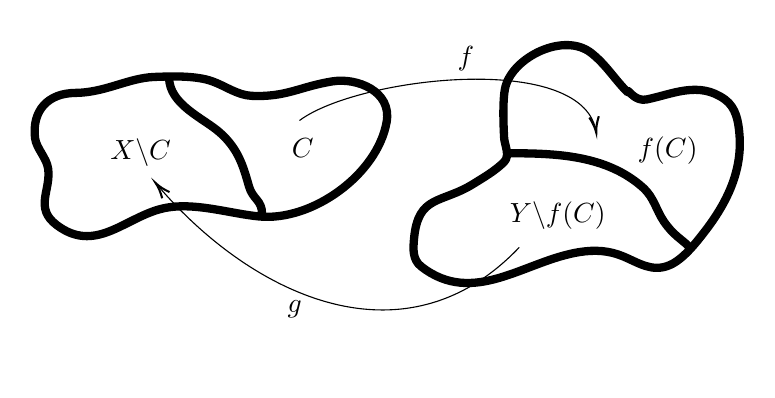
\begin{tikzpicture}[x=0.75pt, y=0.75pt, yscale=-0.7, xscale=0.7]
%uncomment if require: \path (0, 300); %set diagram left start at 0,  and has height of 300

%Shape: Free Drawing [id:dp6757315742756932] 
\draw  [line width=3] [line join = round][line cap = round] (432.84, 94.51) .. controls (423.91, 85.57) and (417.94, 75.44) .. (407.84, 67.51) .. controls (389.3, 52.94) and (354.43, 70.01) .. (348.84, 90.51) .. controls (346.27, 99.93) and (347.79, 123.7) .. (347.84, 125.51) .. controls (348, 130.68) and (352.28, 138.07) .. (347.84, 142.51) .. controls (341.76, 148.59) and (334.14, 152.95) .. (326.84, 157.51) .. controls (304.57, 171.42) and (288.63, 164.83) .. (285.84, 195.51) .. controls (285.19, 202.64) and (284.78, 209.79) .. (290.84, 214.51) .. controls (326.9, 242.55) and (362.17, 210.37) .. (399.84, 204.51) .. controls (410.54, 202.84) and (420.13, 203.46) .. (429.84, 207.51) .. controls (440.63, 212) and (449.78, 218.68) .. (461.84, 213.51) .. controls (471.26, 209.47) and (480.29, 197.67) .. (485.84, 190.51) .. controls (501.13, 170.76) and (511.94, 148.7) .. (509.84, 123.51) .. controls (509.11, 114.78) and (507.62, 105.16) .. (499.84, 99.51) .. controls (481.9, 86.46) and (463.43, 95.99) .. (445.84, 99.51) .. controls (438.37, 101) and (433.82, 93.51) .. (432.84, 93.51) ;
%Shape: Free Drawing [id:dp6453905503802386] 
\draw  [line width=3] [line join = round][line cap = round] (350.84, 136.51) .. controls (383.1, 136.51) and (418.59, 137.55) .. (443.84, 160.51) .. controls (450.93, 166.95) and (452.72, 176.06) .. (457.84, 183.51) .. controls (464.34, 192.96) and (469.88, 195.54) .. (474.84, 200.51) .. controls (475.08, 200.74) and (474.84, 201.17) .. (474.84, 201.51) ;
%Shape: Free Drawing [id:dp051216671495937005] 
\draw  [line width=3] [line join = round][line cap = round] (53, 95) .. controls (33.78, 95) and (22.79, 107.25) .. (25, 126) .. controls (25.84, 133.12) and (32.95, 139.65) .. (34, 147) .. controls (36.15, 162.06) and (24.12, 174.09) .. (40, 186) .. controls (66.02, 205.52) and (85.93, 181.84) .. (111, 175) .. controls (132.29, 169.19) and (157.62, 177.86) .. (179, 180) .. controls (215.66, 183.67) and (260.62, 151.15) .. (267, 115) .. controls (270.77, 93.64) and (246.36, 84.44) .. (230, 87) .. controls (207.33, 90.54) and (198.2, 98.1) .. (174, 97) .. controls (164.41, 96.56) and (156.03, 90.25) .. (147, 87) .. controls (135.47, 82.85) and (118.31, 83.57) .. (107, 84) .. controls (89, 84.69) and (73.05, 95) .. (52, 95) ;
%Shape: Free Drawing [id:dp8803974418610332] 
\draw  [line width=3] [line join = round][line cap = round] (117.26, 84.32) .. controls (117.26, 103.03) and (141.03, 112.34) .. (152.26, 122.32) .. controls (165.02, 133.66) and (168.29, 145.45) .. (172.26, 159.32) .. controls (174.86, 168.42) and (181.26, 168.66) .. (181.26, 178.32) ;
%Curve Lines [id:da948169565487457] 
\draw    (207, 114) .. controls (246.6, 84.3) and (400.4, 66) .. (410.98, 120.64) ;
\draw [shift={(411.26, 122.32)},  rotate = 262.22] [color={rgb,  255:red,  0; green,  0; blue,  0 }  ][line width=0.75]    (10.93, -3.29) .. controls (6.95, -1.4) and (3.31, -0.3) .. (0, 0) .. controls (3.31, 0.3) and (6.95, 1.4) .. (10.93, 3.29)   ;
%Curve Lines [id:da6547582412802545] 
\draw    (358.26, 201.32) .. controls (278.66, 284.9) and (173.32, 233.83) .. (108.97, 158.14) ;
\draw [shift={(108, 157)},  rotate = 49.9] [color={rgb,  255:red,  0; green,  0; blue,  0 }  ][line width=0.75]    (10.93, -3.29) .. controls (6.95, -1.4) and (3.31, -0.3) .. (0, 0) .. controls (3.31, 0.3) and (6.95, 1.4) .. (10.93, 3.29)   ;

% Text Node
\draw (200, 124.4) node [anchor=north west][inner sep=0.75pt]    {$C$};
% Text Node
\draw (314, 61.4) node [anchor=north west][inner sep=0.75pt]    {$f$};
% Text Node
\draw (438, 123.4) node [anchor=north west][inner sep=0.75pt]    {$f( C)$};
% Text Node
\draw (75, 124.4) node [anchor=north west][inner sep=0.75pt]    {$X\backslash C$};
% Text Node
\draw (350, 168.4) node [anchor=north west][inner sep=0.75pt]    {$Y\backslash f( C)$};
% Text Node
\draw (197, 236.4) node [anchor=north west][inner sep=0.75pt]    {$g$};


\end{tikzpicture}
    \end{center}
\end{figure}



\begin{theoremenv}[Cantor-Bernstein]
    Let $X$ and $Y$ be sets. Assume that there exists injective mappings $f:X\rightarrow Y$ and $g:Y\rightarrow X$. Then $X$ and $Y$ are equipotent.
\end{theoremenv}
\begin{proofenv}
    Consider $\Phi:\wp(X)\rightarrow\wp(X), A\mapsto X\backslash g(Y\backslash f(A))$. If $(A, B)\in \wp(X)^2$ such that $A\subseteq B$,  then $f(A)\subseteq f(B), Y\backslash f(A)\supseteq  Y\backslash f(B), g(Y\backslash f(A))\supseteq g(Y\backslash f(A)) , \Phi(A)\subseteq\Phi(B)$. So $\Phi$ is increasing. By Knaster-Tarski theorem,  $\exists C\in \wp(X), C=\Phi(C)$. Then $h:X\rightarrow Y, h(x):=\left\{\begin{matrix}
 f(x), x\in C\\
g^{-1}(x), x\in X\backslash C

\end{matrix}\right.$
is a bijection.
\end{proofenv}

\begin{lemmaenv}
    Let $(X, \le)$ is a partially ordered set.
    \newline
    (1) Let $(A, B)\in \wp(X)^2$,  if $A\subseteq B$,  then $B^\mathrm{u}\subseteq A^\mathrm{u}, B^\mathrm{l}\subseteq A^\mathrm{l}$.
    \newline
    (2) $\forall A\in \wp(X), A\subseteq (A^\mathrm{u})^\mathrm{l}\cap (A^\mathrm{l})^\mathrm{u}$.
\end{lemmaenv}

\begin{theoremenv}[Dedekind-MacNeille]
    \quad
    \newline
    Let $(X, \le )$ be a partially ordered set. Let $\hat{X}:=\{A\in \wp (X)\mid (A^\mathrm{u})^\mathrm{l}=A\}$
\newline
(1) $(\hat{X}, \subseteq)$ is order complete.
\newline
(2) $\forall A\in \wp(X), A^\mathrm{l}\in \hat{X}$.
\newline
(3) $X\rightarrow \hat{X}, x\mapsto \{x\}^\mathrm{l}$ is strictly increasing.
\newline
(4) $\forall A\in \hat{X}$ one has $A=\bigcup_{x\in A}\{x\}^\mathrm{l}=\bigcup_{x\in A}\hat{x}$. In particular,  
$$A=\sup_{(\hat{X}, \subseteq)}\{\hat{x}\mid x\in A\}.$$
(5) Let $A\in \hat{X}$. If $A^\mathrm{u}=\varnothing$,  then $A=X$. If $A^\mathrm{u}\not=\varnothing$, then 
$$A=\bigcap_{x\in A^\mathrm{u}}\hat{x}=\inf_{(\hat{X}, \subseteq)}\{\hat{x}\mid x\in A^\mathrm{u}\}, $$
$$A=\bigcup_{x\in A}\hat{x}=\sup_{(\wp(X), \subseteq)}\{\hat{x}\mid x\in A\}=\sup_{(\hat{X}, \subseteq)}\{\hat{x}\mid x \in A\}.$$
\end{theoremenv}
\begin{remark}
    We've know that $(\wp(X), \subseteq)$ is order complete. So for the sets not order complete,  we can build a relation between them to make it become order complete. And this theorem tell us how to do.
\end{remark}
\begin{proofenv}
    \quad
    \newline
    (1) Consider $\Phi :\wp(X)\rightarrow\wp(X), A\mapsto(A^\mathrm{u})^\mathrm{l}$. By the lemma,  $\Phi $  is increasing. Since $\wp(X)$ is complete, and $\hat{X}$ is the set of fixed point of $\Phi$. By Knaster-Tarski fixed point theorem, $(\hat{X}, \subseteq)$ is order complete.
    \newline
    (2) Let $A\in \wp(X)$,  we prove that $A^\mathrm{l}=((A^\mathrm{l})^\mathrm{u})^\mathrm{l}$. Since $A\subseteq (A^\mathrm{l})^\mathrm{u}$ (by the lemma),  $((A^\mathrm{l})^\mathrm{u})^\mathrm{l}\subseteq A^\mathrm{l}$,  by (2) of the lemma applied to $A^\mathrm{l}$. Hence $A^\mathrm{l}=((A^\mathrm{l})^\mathrm{u})^\mathrm{l}$
    \newline
    (3) Let $x$ and $y$ be element of $X$ such that $x< y$ then $\{x\}^\mathrm{l}\subseteq\{y\}^\mathrm{l}$. In fact,  if $z\in \{x\}^\mathrm{l}, z\le x$. Since $x<y, z<y$. Moreover,  $y\in \{y\}^\mathrm{l}$,  but $y\notin \{x\}^\mathrm{l}$.
    \newline
    (4) $\forall x \in A, x\in \{x\}^\mathrm{l}=\hat{x}$. So $A\subseteq\bigcup_{x\in A}\hat{x}$.
    Conversely,  $\forall x\in A,  x=\min (\{x\}^\mathrm{u})$. Hence $\{x\}^\mathrm{l}=(\{x\}^\mathrm{u})^\mathrm{l}\subseteq (A^\mathrm{u})^\mathrm{l}=A$. Therefore $\bigcup_{x\in A}\{x\}^\mathrm{l}\subseteq A$. Finally we get $\bigcup_{x\in A}\hat{x}=A\in \hat{X}$.
    \newline
    (5) If $A^\mathrm{u}=\varnothing$ then $A=(A^\mathrm{u})^\mathrm{l}=\varnothing^\mathrm{l}=X$. We assume that $A^\mathrm{u}\not=\varnothing$.
    $$\inf _{(\wp(X), \subseteq)}\{\hat{x}|x\in A^\mathrm{u}\}=\bigcap_{x\in A^\mathrm{u}}\hat{x}=\bigcap_{x\in A^\mathrm{u}}\{x\}^\mathrm{l}=(A^\mathrm{u})^\mathrm{l}=A.$$
    So it is equal to $\inf_{(\hat{X}, \subseteq)}\{\hat{x}|x\in A ^\mathrm{u}\}$.
\end{proofenv}
\begin{remark}
    $\forall A\in \hat{X}, A=\{x\in X|\hat{x}\subseteq A\}, A^\mathrm{u}=\{x\in X|A\subseteq \hat{x}\}$.
\end{remark}
\begin{definitionenv}
    $\hat{X}$ is called the Dedekind-MacNeille order completion of $(X, \le)$.
\end{definitionenv}
\section{Recursive Construction}
\begin{definitionenv}
    Let $(X, \le)$ be a partially ordered set. Let $I\subseteq X$. If $\forall a\in I , X_{<a}\subseteq I$,  we say that $I$ is an initial segment of $X$. 
\end{definitionenv}
\begin{propositionenv}
    Let $(X, \le)$ be a totally ordered set,  $I, J$ be initial segments of $X$. Either $I\subseteq J$ or $J\subseteq I$.
\end{propositionenv}
\begin{proofenv}
    Assume that $I\backslash J\not=\varnothing$, take $x\in I\backslash J, \forall y\in J$,  if $y\not\le x $, then $x<y$ and hence $x\in X_{<y}\subseteq J$, contradiction. Therefore $y\le x$. Then $y=x\in I$ or $y\in X_{<x}\subseteq I$.
\end{proofenv}
\begin{propositionenv}
    Let $(X, \le)$ be a well-ordered set. $I$ be an initial segment of $X$,  such that $I\not=X$. There is a unique $a\in X$ such that $I=X_{<a}$.
\end{propositionenv}
\begin{proofenv}
    $X\backslash I\not=\varnothing$ Let $a=\min (X\backslash I)$. By definition, $I\subseteq X_{<a}$. In fact,  $\forall y\in I$ if $y\not< a $,  then $a\le y$.
    Since $I$ is an initial segment $a\in I$,  contradiction.
    \newline
    Conversely,  if $x\in X_{<a}$,  then $x\notin X\backslash I$. Since otherwise $a\le x$. Therefore $x\in I$. Uniqueness, $\forall a\in X, a=\min(X\backslash X_{<a})=\min(X_\leq a)$. Hence $X_{<a}=X_{<b}\Rightarrow a=b$.
\end{proofenv}
\begin{propositionenv}
    Let $(X, \le)$ be a partially ordered set,  $\Lambda$ be a non-empty set,  and $(I_\lambda)_{\lambda\in \Lambda}$ be a family of initial segments of $X$. Then 
    $$I:=\bigcap_{\lambda\in \Lambda}I_\lambda, \space J:=\bigcup_{\lambda\in \Lambda}I_\lambda$$ are initial segments of $X$.
\end{propositionenv}
\begin{proofenv}
    \quad
    \newline
    Let $a\in I.\forall \lambda\in \Lambda, a\in I_\lambda$ and hence $X_{<a}\subseteq I_\lambda$. Therefore, $X_{<a}\subseteq\bigcap_{\lambda\in\Lambda}I_\lambda=I$.
    \newline
    Let $b\in J$.Then $\exists \lambda_0\in \Lambda$ such that $b\in I_{\lambda_0}$. So $X_{<b}\subseteq I_{\lambda_0}\subseteq \bigcup_{\lambda\in \Lambda}I_\lambda=J$. 
\end{proofenv}
\begin{theoremenv}[Recursive construction]
    Let $(X, \le)$ be a well ordered set,  and $Y$ be a set. For any $x\in X$ and any mapping $h:X_{<x}\rightarrow Y$,  we fix an element $\Phi(h)\in Y$. Then,  there exists a unique mapping $f:X\rightarrow Y$  such that 
    $$\forall x\in X,  f(x)=\Phi(f\mid_{X_{<x}}).$$
\end{theoremenv}
\begin{exampleenv}
    For any $(a_0, \dots, a_{n-1})\in \RR^n$,  we fix an element $a_{n-1}+\varepsilon\in \RR$,  where $\varepsilon$ is a real number. There exists a unique mapping $(n\in \NN)\mapsto f(n)$ such that $f(n)=f(n-1)+\varepsilon$.($f(n):=n\varepsilon$).
\end{exampleenv}
\begin{proofenv}
    \quad
    \newline
    ``Uniqueness": 
    \newline
    Let $f, g$ be mappings from $X$ to $Y$ such that 
    $$\forall x\in X, f(x)=\Phi(f\mid_{X_{<x}}), g(x)=\Phi(g\mid_{X_{<x}}).$$
    Then: $\forall x\in X$,  we have 
    $$(\forall y\in X_{<x}, f(y)=g(y))\Rightarrow f(x)=g(x).$$
    So by inclusion $\forall x \in X,  f(x)=g(x)$,  namely,  $f=g$.
    \newline
    ``Existence": 
    \newline
    Let $\mathscr{S}$  be the set of initial segments $S$ of $X$ such that $\exists f_S:S\rightarrow Y$ satisfying 
    \begin{equation*}
        \forall x\in S, f_S(x)=\Phi(f_S\mid_{X_{<x}}). \tag{$*$}
    \end{equation*}
    Let $X_0=\bigcup_{S\in\mathscr{S} }S$. It is also an initial segment of $X$. For any $x\in X_0$ there exists $ S $ such that $x\in S$. If $S_1$ and $S_2$ are two elements of $\mathscr{S}$,  then $S_1\cap S_2$ is also an initial segment. Moreover $f_{S_1}\mid_{S_1\cap S_2}$ and $f_{S_2}\mid_{S_1\cap S_2}$ satisfy $(*)$ So $f_{S_1}\mid_{S_1\cap S_2}=f_{S_2}\mid_{S_1\cap S_2}$. Thus $f_S(x)$ does not depend on the choice of $S\in \mathscr{S}$ containing $x$. We denote it as $f(x)$. $f:X_0\rightarrow Y$ satisfying $(*)$. So $X_0\in \mathscr{S}$.
    If $X_0\not=X.\exists a\in X$ such that $ X_0=X_{<a}$. We extend $f$ to $X_0\cup\{a\}$ by letting $f(a)=\Phi(f)$. Then we get $X_0\cup\{a\}\in \mathscr{S}$.Contradiction.Therefore $X_0=X$  and we get the existence of $f$. 
\end{proofenv}

\begin{definitionenv}
    Let $A$ be a set. If there exists an injective mapping $A\rightarrow \NN$,  then we say that $A$ is \textbf{countable}.
    If  there exists an injective mapping $f:A\rightarrow \NN$ such that $f(A)$ is bounded from above (having an upper bound in $\NN$),  then we say that $A$ is \textbf{finite}.
\end{definitionenv}
\begin{lemmaenv}\label{4.9.8}
    \quad
    \newline
    (1) Let $n\in \NN$ and $x_0, \dots , x_n$ be elements of $\NN$ such that $x_0<\dots<x_n$,  then $\forall i\in \NN_{\leq n}, i\leq x_i$.
    \newline
    (2) Let $(x_n)_{n\in \NN}$ be a family of elements in $\NN$ such that $\forall n\in \NN, x_n<x_{n+1}$,  then $\forall i\in \NN, i\le x_i$.
\end{lemmaenv}
\begin{proofenv}
    If $j\le x_j$ for $j\in \{0, \dots, i-1\}$. Then,  in the case where $i=0, 0\le x_0$ holds since $0=\min_\le \NN$. In the case where $i>0$,  one has $i-1\le x_{i-1}<x_i$. So $x_i\ge x_{i-1}+1\ge i-1+1=i$.
\end{proofenv}
\begin{propositionenv}
    Let $f:A\rightarrow B$ be a mapping.
    \newline
    (1) If $f$ is injective and if $B$ is finite,  then $A$ is finite.(resp. countable)
    \newline
    (2) If $f$ is surjective and $A$ is finite,  then $B$ is finite.(resp countable)
\end{propositionenv}
\begin{proofenv}
    \quad
    \newline
    (1) Let $g:B\rightarrow \NN$ injective and bounded from above. Then $g\circ f$ is injective and $\mathrm{Im}(g\circ f)\subseteq \mathrm{Im}(g)$.
    \newline
    (2) $\exists$ injective mapping $B\rightarrow A$ by the axiom of choice. $f:A\rightarrow B$ For any $b\in B$,  pick $h(b)\in f^{-1}(\{b\})\subseteq A$, $h:B\rightarrow A$. If $h(b)=h(b')$,  then $f(h(b))=f(h(b'))=b'$.
\end{proofenv}
\begin{propositionenv}
    Let $X, Y$ be sets.
    \newline
    (1) If $X$ and $Y$ are finite,  then $X\cup Y$ is finite.(resp. countable)
    \newline
    (2) If $X$ is infinite and $Y$ is finite,  then $X\backslash Y$ is infinite.(resp. uncountable)
\end{propositionenv}
\begin{proofenv}
    \quad
    \newline
    (1) Let $f:X\rightarrow \NN$ and $g:Y\rightarrow \NN$ be injective mappings. We construct $h:X\cup Y\rightarrow \NN$ such that 
    $$h(x)=\left\{\begin{matrix}
     2f(x)\,  &x\in X\\
    2g(x)+1\, &x\in Y\backslash X

    \end{matrix}\right.$$
    $h$ is then injective,  and $h$ is bounded if $f$ and $g$ are bounded.
    \newline
    In fact,  if $(x, y)\in (X\cup Y)^2$, 
    \newline
    either $(x, y)\in X^2$ and $h(x)=2f(x)=h(y)=2f(y)$ if and only if $x=y$.
    \newline
    or $(x, y)\in (Y\backslash X)^2$ and $h(x)=h(y)\Rightarrow x=y$.
    \newline
    or $x\in X, y\in Y\backslash X.h(x)\not=h(y)$ (So $h(x)=h(y)\Rightarrow x=y$).
    \newline
    or $y\in X, x\in Y\backslash X , h(x)\not=h(y)$.
    \newline
    (2)  Assume that $X\backslash Y$ is finite,  then $X=(X\backslash Y)\cup Y$ is also finite.
\end{proofenv}
\begin{notationenv}
    If $f:X\rightarrow X$  is a mapping. Then $f^0$ denotes $\mathrm{Id}_X$. For $n\in\NN_{\ge 1}$, $f^n$ denotes $\underset{n}{\underbrace{f\circ f\circ \dots \circ f}}$. 
\end{notationenv}
\begin{theoremenv}\label{4.9.12}
    $\NN\times\NN$ and $\NN$ are equipotent.
\end{theoremenv}
\begin{proofenv}
    Let $f:\NN\times\NN\rightarrow \NN, (a, b)\mapsto2^a(2b+1)$. It is an injective mapping since $2^a(2b+1)=2^{a'}(2b'+1)$.So $a=a', b=b'$.Moreover $x\mapsto(0, x)$ is injective.
\end{proofenv}
\begin{corollaryenv}
    $\forall n\in \NN,  n\ge 1, \NN^n$ and $\NN$ are equipotent.
\end{corollaryenv}
\begin{proofenv}
    Induction on $n$.
    \newline
    For $n=1$,  easy. We assume that $\NN^n$ is equipotent to $\NN$ and $f:\NN^n\rightarrow\NN$ be a bijection. Then the mapping
    $$f':\NN^n\times \NN\rightarrow \NN\times\NN, \, \left(x_1, \dots, x_n;x_{n+1}\right)\mapsto\left(f(x_1, \dots, x_n), x_{n+1}\right)$$ 
    is a bijection. By Theorem \ref{4.9.12},  there exists a bijection $g:\NN^2\rightarrow\NN$.Therefore, 
    $$g\circ f':\NN^{n+1}\rightarrow\NN$$
    is a bijection,  which leads to $\NN^{n+1}$ and $\NN$ are equipotent.
\end{proofenv}

\textbf{Motivation}: Let $X$ be a set. A sequence in $X$ is by definition a family $(x_i)_{i\in I}$,  where $I$ is an infinite subset of $\NN$,  and each $x_i$ is an element of $X$.
\begin{exampleenv}
    $(a+bn)_{n\in \NN};\left(\frac{1}{n}\right)_{n\in \NN_{\ge 1}}$.
\end{exampleenv}
\begin{propositionenv}
    Let $I\subseteq \NN$.
    \newline
    (1) $\mathrm{Id}_I:I\rightarrow I$ is the only increasing mapping bijection from $I$ to $I$.
    \newline
    (2) If $I$ is bounded from above,  then $\mathrm{Id}_I$ is the only strictly increasing mapping from $I$ to $I$.
\end{propositionenv}
\begin{proofenv}
    \quad
    \newline
    (1) Let $f:I\rightarrow I$ be an increasing bijection. We want to prove:
    $$A:=\{x\in I\mid f(x)\not=x\}=\varnothing.$$
    If this set is non-empty,  it has a least element $n_0$. By definition,  $f(n_0)\not=n_0$. So either $n_0<f(n_0)$ or $n_0>f(n_0)$.
    \newline
    If $f(n_0)<n_0$,  then $f(n_0)\notin A$,  and hence $f(n_0)=f(f(n_0))<f(n_0)$,  contradiction. So $n_0<f(n_0)$. For any $n\in I$,  if $n_0\le n$ then $f(n_0)\le f(n)$. If $n_0>n$,  then $n\notin A$ and $f(n)=n<n_0$.$(*)$Hence $f(n)\not=n_0$ for any $n\in I$. This contradicts the assumption that $f$ is bijective.
    \newline
    (2) Suppose that $I$ is bounded from above,  and $f:I\rightarrow I$ is strictly increasing. We follow the same reasoning until $(*)$. $n_0<f(n_0)$ implies that $\forall k \in \NN,  f^k(n_0)<f^{k+1}(n_0)$,  that means 
    $$n_0<f(n_0)<\dots <f^{k+1}(n_0).$$
    So by the lemma \ref{4.9.8},  $k\le f^k(n_0)$,  this contradicts the assumption that $I$ is bounded from above.
\end{proofenv}
\begin{corollaryenv}
    Let $I\subseteq \NN$ bounded from above,  and $J\subseteq I$.If $J\not=I$,  there does not exist a strictly increasing mapping from $I$ to $J$.
\end{corollaryenv}
\begin{proofenv}
    Suppose that $f:I\rightarrow J$ is a strictly increasing mapping. Let $g:J\rightarrow I, x\mapsto x$ be a inclusion mapping. So $g\circ f:I\rightarrow I$ is strictly increasing and hence $g\circ f=\mathrm{Id}_I$. However $\mathrm{Im}(g\circ f)\subseteq\mathrm{Im}(g)=J\not=I$. Contradiction.
\end{proofenv}
\begin{propositionenv}
    Let $I\subseteq \NN$ non-empty.
    \newline
    (1) If $I$ is bounded from above,  then there exists a unique pair $(N, f)$,  where $N\in \NN$ and $f:\{0, 1, \dots, N\}\rightarrow I$ is an increasing bijection. (We say that the cardinality of $I$ is $N+1$.)
    \newline
    (2) If $I$ is NOT bounded from above,  there exists an increasing bijection from $\NN$ to $I$. (We say that the cardinality of $I$ is $\aleph_0$) 
\end{propositionenv}
\begin{proofenv}
    \quad
    \newline
    We construct in a recursive way a family of elements in $I$. Let $x_0=\min(I)$. If $x_0, \dots , x_n$ are chosen (with $x_0<\dots<x_n$) we pick $x_{n+1}=\min(I\backslash\{x_0, \dots, x_n\})$. We slop at $N$ if $\{x_0, \dots, x_N\}=I$. Thus we obtain the increasing bijection needed by the proposition.
    \newline
    ``Uniqueness" for (2): If $f:\NN\rightarrow I, g:\NN\rightarrow I$ are increasing bijections,  then $f^{-1}\circ g:\NN\rightarrow\NN$ and $g^{-1}\circ f:\NN\rightarrow\NN$ are increasing bijections. So $f^{-1}\circ g=\mathrm{Id}_{\NN}$. Hence $f=g$.
    \newline
    ``Uniqueness" for (1): Let $f:\{0, 1, \dots, N\}\rightarrow I$ and $g:\{0, 1, \dots, M\}\rightarrow I$ be increasing bijections. $g^{-1}\circ f:\{0, 1, \dots, N\}\rightarrow \{0, 1, \dots,  M\}$ and $g:\{0, 1, \dots, M\}\rightarrow I$ be increasing bijections. $f^{-1}\circ g:\{0, 1, \dots, M\}\rightarrow \{0, 1, \dots,  N\}$ are increasing bijection. So $N\le M$ and $M\le N$,  which leads to $N=M, g=f$. 
\end{proofenv}
\begin{corollaryenv}
    A non-empty set $X$ is finite if and only if it can be written as $\{x_0, \dots, x_N\}$ where $N\in \NN$,  and $x_0, \dots, x_N$ are distinct elements of $X$.
\end{corollaryenv}
\begin{proofenv}
    Let $f:X\rightarrow \NN$ be an injective mapping with $f(x)$ bounded from above. Then there exists $(N, g)$ where $N\in \NN$ and $g:\{0, \dots , N\}\rightarrow f(x)$ is an increasing bijection. Then $f^{-1}\circ g:\{0, \dots, N\}\rightarrow X$ is a bijection. We take $x_i$ to be $(f^{-1}\circ g)(i)$ (Note that $N$ is unique $N+1$ is called the cardinality of $X$).
\end{proofenv}
\begin{propositionenv}
    Let $X$ be a set. The following condition are equipotent:
    \newline
    (1) $X$ is infinite.
    \newline
    (2) $\exists \NN\rightarrow X$ injective.
    \newline
    (3) $\exists$ injective mapping $f:X\rightarrow X$ such that $f(X)\not=X$.
\end{propositionenv}
\begin{proofenv}
    \quad
    \newline
    (1)$\Rightarrow$(2) We construct a sequence $(x_n)_{n\in \NN}$ in $X$ as follows. $X\not=\varnothing$. We pick arbitrary $x_0\in X$. Suppose that distinct elements $x_0, \dots,  x_n$ of $X$ are chosen. The set $X\backslash\{x_0, \dots, x_n\}\not=\varnothing$ since otherwise $X=\{x_0, \dots, x_n\}$ is finite. We pick $x_{n+1}\in X\backslash\{x_0, \dots, x_n\}, \,  x_0, \dots, x_{n+1}$ are distinct. The mapping $\NN\rightarrow X,  n\mapsto x_n$ is injective.
    \newline
    (2)$\Rightarrow$(3) Let $f:\NN\rightarrow X$ be injective. We define $g:X\rightarrow X$.
    $$g(x):=
\left\{\begin{matrix}
 f(n+1)&,  &x=f(n) \\
x&, &x\notin f(\NN).
\end{matrix}\right. $$
$g(X)\not=X$ since $f(0)\notin g(X)$ If $x\notin f(\NN), g(x)=x\notin f(\NN)$,  so $g(x)\not=f(0)$. If $x=f(n),  g(x)=f(n+1)\not=f(0)$ since $f$ is injective.
\newline
(3)$\Rightarrow$(2) Let $g:X\rightarrow X$ be injective with $g(X)\not=X$. We pick $x_0\in X\backslash g(X)$. We define a sequence $(x_n)_{n\in\NN}$ by letting $x_{n+1}:=g(x_n)$. Since $g$ is injective,  $x_n\in g^n(X)\backslash g^{n+1}(X)$. otherwise $\exists y\in X$,  such that $x_n=g^{n}(x_0)=g^{n+1}(y)$. Hence $x_0=g(y)\in g(x)$ contradiction. Then $x_0, x_1, \dots, $ are distinct,  which defines an injective mapping $\NN\rightarrow X, n\mapsto x_n$.
\newline
(2)$\Rightarrow$(1) If $X$ is finite,  $\exists g:X\rightarrow\NN$ injective with $g(x)$ bounded. Then $\NN\rightarrow X\overset{g}{\rightarrow}\NN$ is injective with $h(\NN)$ bounded from above.
\end{proofenv}